\documentclass{standalone}
\usepackage{tikz}
\usepackage{amsmath}
\usetikzlibrary{decorations.markings}

\begin{document}
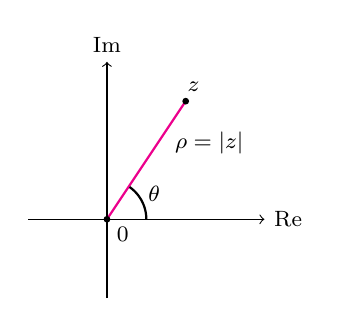
\begin{tikzpicture}
  \draw[->] (-1,0) -- (2,0) node[right] {\footnotesize$\operatorname{Re}$};
  \draw[->] (0,-1) -- (0,2) node[above] {\footnotesize$\operatorname{Im}$};
  


\draw[magenta, thick] (0,0) -- (1,1.5);
\node[anchor=south] at (1.3,0.7) {\footnotesize$\rho = |z|$};


   \filldraw (1,1.5) circle (1pt);
    \node[anchor=south] at (1.1,1.5) {\footnotesize$z$};
  
  
  
  \filldraw (0,0) circle (1pt);
  \node[anchor=south] at (0.2,-0.4) {\footnotesize$0$};
  
  
   \draw [thick,domain=0:55] plot ({0.5*cos(\x)}, {0.5*sin(\x)});


  \node[anchor=south] at (0.6,0.1) {\footnotesize$\theta$};
    
\end{tikzpicture}
\end{document}